\documentclass[12pt]{article}
\usepackage{amsmath, amssymb}
\usepackage{graphicx}
\usepackage{tikz}
\usepackage{hyperref}
\usepackage{caption}
\usepackage{float}
\usepackage[margin=1in]{geometry}

\title{Quantum Mechanics Foundations for Quantum Computing}
\author{Quantum Computing Course \\ Computer Science Department}
\date{Lecture 2: Physical Principles}

\begin{document}

\maketitle

\section*{Introduction}
This lecture introduces the fundamental quantum mechanical principles that form the physical basis for quantum computing. We will focus on concepts rather than mathematical formalism, with emphasis on how these principles enable the creation and manipulation of qubits.

\section{Wave-Particle Duality}

\subsection{The Double-Slit Experiment}

\begin{figure}[H]
    \centering
    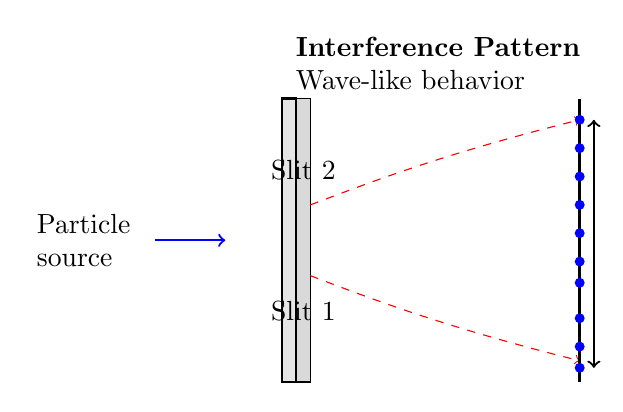
\begin{tikzpicture}[scale=0.9]
        % Barrier
        \draw[thick, fill=gray!20] (-0.2,0) rectangle (0,4);
        \draw[thick] (0,1.5) -- (0.2,1.5);
        \draw[thick] (0,2.5) -- (0.2,2.5);
        \draw[fill=gray!30] (0,0) rectangle (0.2,4);
        \node at (0.1,1) {Slit 1};
        \node at (0.1,3) {Slit 2};
        
        % Particle source
        \draw[->, thick, blue] (-2,2) -- (-1,2);
        \node[align=left] at (-3,2) {Particle\\source};
        
        % Paths through slits
        \draw[dashed, ->, red] (0.2,1.5) .. controls (1,1.2) and (2,0.8) .. (4,0.3);
        \draw[dashed, ->, red] (0.2,2.5) .. controls (1,2.8) and (2,3.2) .. (4,3.7);
        
        % Detection screen
        \draw[very thick] (4,0) -- (4,4);
        
        % Interference pattern dots
        \foreach \y in {0.2,0.5,0.9,1.4,1.7,2.1,2.5,2.9,3.3,3.7} {
            \fill[blue] (4,\y) circle (2pt);
        }
        
        % Labels
        \node[align=left] at (2,4.5) {\textbf{Interference Pattern}\\Wave-like behavior};
        \draw[<->, thick] (4.2,0.2) -- (4.2,3.7);
    \end{tikzpicture}
    \caption{Double-slit experiment showing wave-like interference pattern. Individual particles build up an interference pattern over time.}
    \label{fig:double-slit}
\end{figure}

\subsubsection{Experimental Observations}

The double-slit experiment reveals the fundamental wave-particle duality of quantum systems:

\begin{enumerate}
    \item \textbf{Particles sent one at a time:} Even when individual particles (electrons or photons) are sent through the apparatus, an interference pattern gradually builds up on the detection screen.
    
    \item \textbf{Which-path information:} If we place detectors at the slits to determine which path each particle takes, the interference pattern disappears and we see two distinct bands.
    
    \item \textbf{Wave-like behavior:} The interference pattern indicates that each particle behaves as if it passes through \textit{both slits simultaneously} and interferes with itself.
\end{enumerate}

\subsubsection{Key Implications for Quantum Computing}

\begin{itemize}
    \item \textbf{Superposition:} Quantum systems can exist in multiple states/paths simultaneously.
    \item \textbf{Interference:} Different possibilities can interfere constructively or destructively.
    \item \textbf{Measurement effect:} The act of measurement fundamentally changes the system's behavior.
    \item \textbf{Quantum parallelism:} A quantum system can explore multiple computational paths simultaneously.
\end{itemize}

\section{Creating Qubits: Physical Implementations}

\subsection{Electron-Based Qubits (USA/Europe Approach)}

\begin{figure}[H]
    \centering
    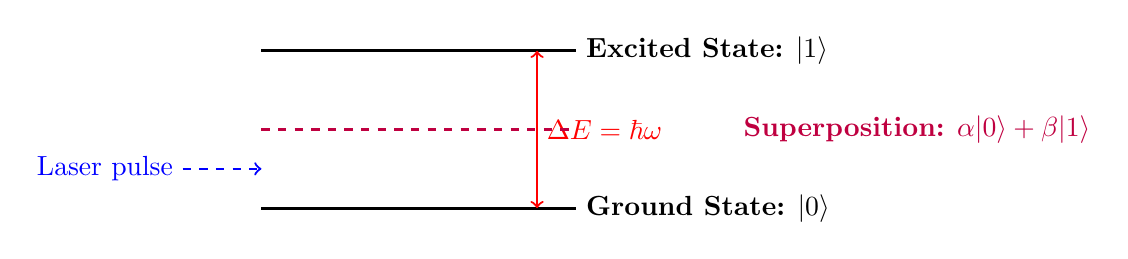
\begin{tikzpicture}[scale=1.0]
        % Energy levels
        \draw[very thick] (-2,0) -- (2,0);
        \node[right] at (2,0) {\textbf{Ground State:} $|0\rangle$};
        
        \draw[very thick] (-2,2) -- (2,2);
        \node[right] at (2,2) {\textbf{Excited State:} $|1\rangle$};
        
        % Energy gap
        \draw[<->, thick, red] (1.5,0) -- (1.5,2);
        \node[right, red] at (1.5,1) {$\Delta E = \hbar \omega$};
        
        % Laser excitation
        \draw[->, thick, blue, dashed] (-3,0.5) -- (-2,0.5);
        \node[left, blue] at (-3,0.5) {Laser pulse};
        
        % Superposition state
        \draw[dashed, thick, purple] (-2,1) -- (2,1);
        \node[right, purple] at (4,1) {\textbf{Superposition:} $\alpha|0\rangle + \beta|1\rangle$};
        
        % System representation
        %\draw[fill=orange!20] (0,-1) ellipse (1.5 and 0.5);
        %\node at (0,-1) {Atom/Quantum Dot/Superconducting Circuit};
    \end{tikzpicture}
    \caption{Creating qubits by exciting electrons between discrete energy levels. Precise laser or microwave pulses create superposition states.}
    \label{fig:electron-qubits}
\end{figure}

\subsubsection{Physical Principle}

Electrons in quantum systems occupy discrete energy levels. By applying precisely controlled energy pulses, we can create superposition states:

\begin{itemize}
    \item \textbf{Ground state:} $|0\rangle$ - lowest energy configuration
    \item \textbf{Excited state:} $|1\rangle$ - higher energy configuration
    \item \textbf{Superposition:} $\alpha|0\rangle + \beta|1\rangle$ - coherent combination
\end{itemize}

\subsubsection{Implementation Methods}

\begin{enumerate}
    \item \textbf{Superconducting qubits:} Tiny circuits where electrons flow without resistance, with energy levels quantized.
    \item \textbf{Trapped ions:} Individual atoms suspended in electromagnetic fields, using electron energy levels.
    \item \textbf{Quantum dots:} Nanoscale semiconductor structures that confine electrons in discrete energy levels.
\end{enumerate}

\subsubsection{Key Requirements}

\begin{itemize}
    \item \textbf{Isolation:} System must be isolated from environmental noise.
    \item \textbf{Precise control:} Laser/microwave pulses must have exact frequency and duration.
    \item \textbf{Low temperature:} Often requires cryogenic cooling to reduce thermal noise.
\end{itemize}

\subsection{Photon-Based Qubits (Chinese Approach)}

\begin{figure}[H]
\centering
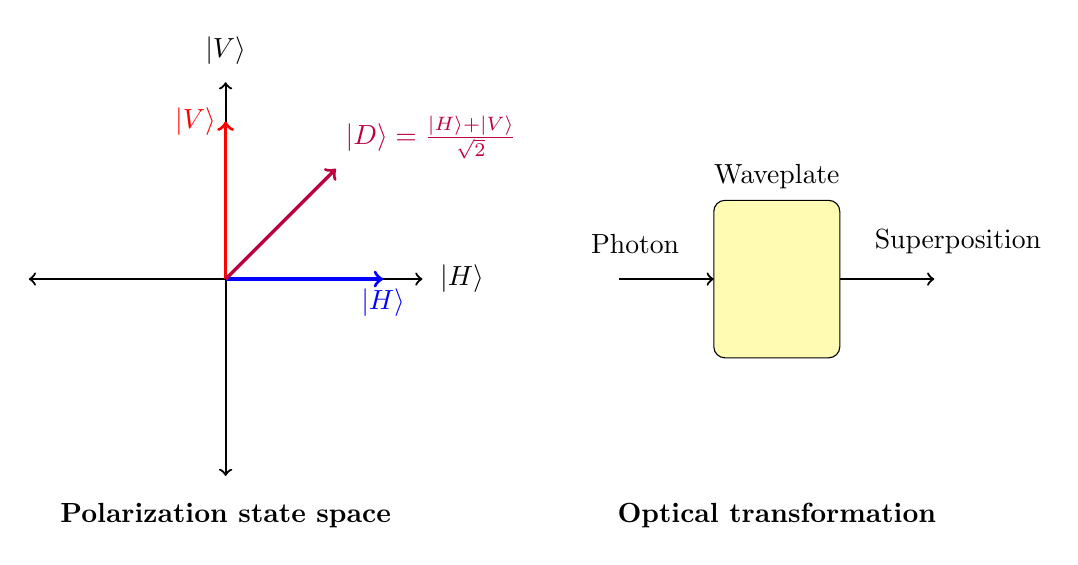
\begin{tikzpicture}[scale=1]

% =========================
% LEFT: Polarization space
% =========================
\begin{scope}[shift={(-4,0)}]

    % Axes
    \draw[<->, thick] (-2.5,0) -- (2.5,0);
    \draw[<->, thick] (0,-2.5) -- (0,2.5);

    % Axis labels
    \node[right] at (2.6,0) {$|H\rangle$};
    \node[above] at (0,2.6) {$|V\rangle$};

    % Basis vectors
    \draw[->, very thick, blue] (0,0) -- (2,0);
    \draw[->, very thick, red] (0,0) -- (0,2);

    % Diagonal state
    \draw[->, very thick, purple] (0,0) -- (1.4,1.4);

    % State labels
    \node[blue, below] at (2,0) {$|H\rangle$};
    \node[red, left] at (0,2) {$|V\rangle$};
    \node[purple, above right] at (1.4,1.4)
        {$|D\rangle=\frac{|H\rangle+|V\rangle}{\sqrt{2}}$};

    % Title
    \node at (0,-3) {\textbf{Polarization state space}};
\end{scope}

% =========================
% RIGHT: Optical process
% =========================
\begin{scope}[shift={(3,0)}]

    % Input photon
    \draw[->, thick] (-2,0) -- (-0.8,0);
    \node[above] at (-1.8,0.2) {Photon};

    % Waveplate
    \draw[fill=yellow!30, rounded corners=4pt]
        (-0.8,-1) rectangle (0.8,1);
    \node at (0,1.3) {Waveplate};

    % Output
    \draw[->, thick] (0.8,0) -- (2,0);
    \node[above] at (2.3,0.2) {Superposition};

    % Title
    \node at (0,-3) {\textbf{Optical transformation}};
\end{scope}

\end{tikzpicture}

\caption{Photon polarization qubit. Left: abstract polarization state space. Right: a waveplate converts an input polarization into a superposition state.}
\label{fig:photon-qubits}
\end{figure}


\subsubsection{Physical Principle}

Photons can be polarized in different directions. The polarization state serves as the qubit:

\begin{itemize}
    \item \textbf{Basis states:} $|H\rangle$ (horizontal), $|V\rangle$ (vertical)
    \item \textbf{Superposition:} $|D\rangle = \frac{1}{\sqrt{2}}(|H\rangle + |V\rangle)$ (diagonal)
    \item \textbf{Phase superposition:} $|R\rangle = \frac{1}{\sqrt{2}}(|H\rangle + i|V\rangle)$ (right circular)
\end{itemize}

\subsubsection{Implementation Methods}

\begin{enumerate}
    \item \textbf{Polarization encoding:} Using waveplates to rotate photon polarization.
    \item \textbf{Path encoding:} Photon taking multiple paths through an interferometer.
    \item \textbf{Time-bin encoding:} Photon arriving at different times.
\end{enumerate}

\subsubsection{Advantages of Photonic Qubits}

\begin{itemize}
    \item \textbf{Low decoherence:} Photons interact weakly with environment.
    \item \textbf{Room temperature operation:} No cryogenic cooling needed.
    \item \textbf{High-speed transmission:} Can be sent through optical fibers.
    \item \textbf{Easy manipulation:} Standard optical components (waveplates, beam splitters).
\end{itemize}

\begin{table}[H]
    \centering
    \begin{tabular}{|p{0.22\textwidth}|p{0.36\textwidth}|p{0.36\textwidth}|}
    \hline
    \textbf{Feature} & \textbf{Electron-based (USA/EU)} & \textbf{Photon-based (China)} \\
    \hline
    Physical system & Atoms, superconducting circuits & Photon polarization/path \\
    Operating temperature & Cryogenic (near 0K) & Room temperature \\
    Gate speed & Nanoseconds & Picoseconds \\
    Decoherence time & Microseconds to milliseconds & Long (weak interaction) \\
    Measurement efficiency & High & Moderate (photon loss) \\
    Scalability challenge & Qubit connectivity & Photon sources/detectors \\
    \hline
    \end{tabular}
    \caption{Comparison of qubit implementation approaches}
    \label{tab:qubit-comparison}
\end{table}

\section{Measurement Collapse to Pure States}

\subsection{The Measurement Postulate}

When a quantum system in superposition is measured, it "collapses" to one of the basis states:

\[
|\psi\rangle = \alpha|0\rangle + \beta|1\rangle \xrightarrow{\text{measure}} 
\begin{cases}
|0\rangle & \text{with probability } |\alpha|^2 \\
|1\rangle & \text{with probability } |\beta|^2
\end{cases}
\]

\begin{figure}[H]
\centering
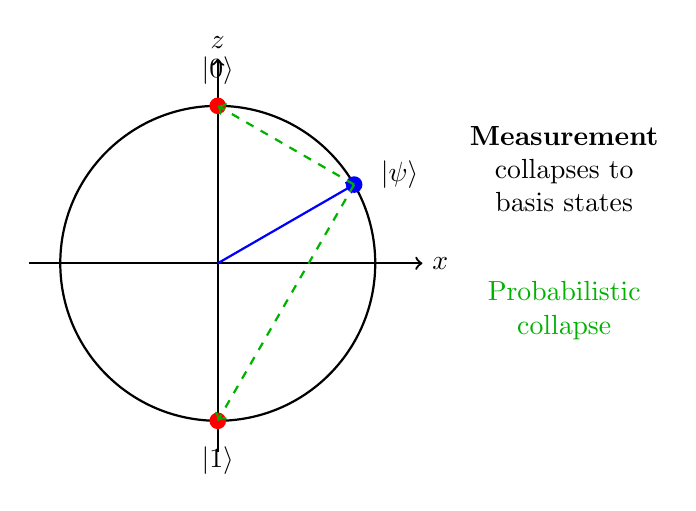
\begin{tikzpicture}[scale=1]

% Bloch sphere
\draw[thick] (0,0) circle (2);

% Axes
\draw[->, thick] (0,-2.4) -- (0,2.6);
\node[above] at (0,2.6) {$z$};

\draw[->, thick] (-2.4,0) -- (2.6,0);
\node[right] at (2.6,0) {$x$};

% Reference radius
\draw[dashed] (0,0) -- (30:2);

% Basis states
\fill[red] (0,2) circle (3pt);
\fill[red] (0,-2) circle (3pt);

\node[above] at (0,2.15) {$|0\rangle$};
\node[below] at (0,-2.2) {$|1\rangle$};

% Superposition state
\fill[blue] (30:2) circle (3pt);
\draw[->, thick, blue] (0,0) -- (30:2);

\node[right] at (30:2.25) {$|\psi\rangle$};

% Measurement collapse arrows
\draw[->, dashed, thick, green!70!black] (30:2) -- (0,2);
\draw[->, dashed, thick, green!70!black] (30:2) -- (0,-2);

% Explanatory labels (moved OUTSIDE sphere)
\node[align=center] at (4.4,1.2)
{\textbf{Measurement}\\collapses to\\basis states};

\node[align=center, green!70!black] at (4.4,-0.6)
{Probabilistic\\collapse};

\end{tikzpicture}
\caption{Measurement on the Bloch sphere. A superposition state $|\psi\rangle$ collapses probabilistically to one of the computational basis states.}
\label{fig:measurement-collapse}
\end{figure}

\subsection{Physical Explanation}

The measurement process involves interaction between the quantum system and a macroscopic measuring device:

\begin{enumerate}
    \item \textbf{System-apparatus interaction:} The quantum system becomes entangled with the measuring device.
    \item \textbf{Decoherence:} Environmental interactions destroy phase coherence between superposition components.
    \item \textbf{Classical outcome:} The measuring device settles into a definite macroscopic state corresponding to one of the quantum basis states.
\end{enumerate}

\subsection{Key Quantum Principles Involved}

\subsubsection{1. Born Rule}
The probability of obtaining a particular measurement outcome is given by the square of the amplitude:
\[
P(i) = |\langle \phi_i | \psi \rangle|^2
\]
where $\{|\phi_i\rangle\}$ is the measurement basis.

\subsubsection{2. Projection Postulate}
After measurement, the state is projected onto the corresponding basis vector:
\[
|\psi\rangle \rightarrow \frac{P_i |\psi\rangle}{\sqrt{\langle \psi|P_i|\psi\rangle}}
\]
where $P_i = |\phi_i\rangle\langle\phi_i|$ is the projection operator.

\subsubsection{3. Repeatability}
Immediate re-measurement yields the same result:
\[
\text{If } |\psi\rangle \xrightarrow{\text{measure}} |\phi_i\rangle, \text{ then } |\phi_i\rangle \xrightarrow{\text{measure}} |\phi_i\rangle
\]

\subsection{Implications for Quantum Computing}

\begin{itemize}
    \item \textbf{Output extraction:} Measurement is how we read computational results.
    \item \textbf{Probabilistic outcomes:} Quantum algorithms often require multiple runs.
    \item \textbf{Basis choice:} Different measurements extract different information.
    \item \textbf{Irreversibility:} Measurement destroys quantum coherence for the measured observable.
\end{itemize}

\section{Quantum Entanglement: Basic Principles}

\subsection{Definition and Creation}

Two or more quantum systems become entangled when their quantum states cannot be described independently:

\[
|\psi\rangle_{AB} \neq |\phi\rangle_A \otimes |\chi\rangle_B
\]

\begin{figure}[H]
\centering
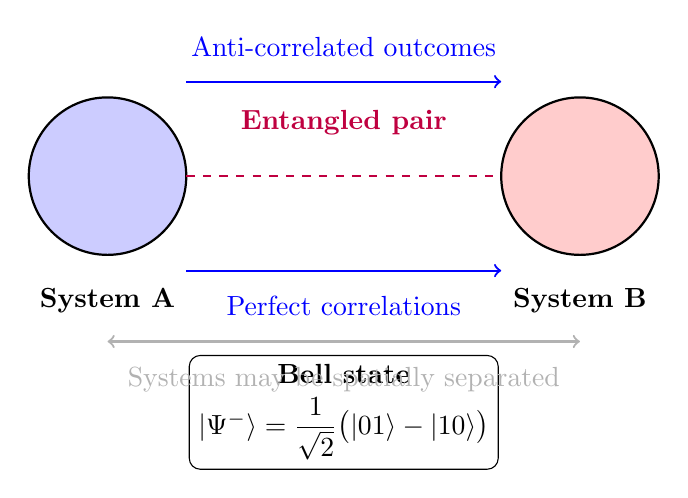
\begin{tikzpicture}[scale=1]

% ======================
% Systems
% ======================
\draw[fill=blue!20, thick] (0,0) circle (1);
\draw[fill=red!20, thick] (6,0) circle (1);

\node[below] at (0,-1.3) {\textbf{System A}};
\node[below] at (6,-1.3) {\textbf{System B}};

% ======================
% Entanglement link
% ======================
\draw[thick, purple, dashed] (1,0) -- (5,0);
\node[purple, above] at (3,0.4) {\textbf{Entangled pair}};

% ======================
% Correlations
% ======================
\draw[->, thick, blue] (1,1.2) -- (5,1.2);
\node[blue, above] at (3,1.4) {Anti-correlated outcomes};

\draw[->, thick, blue] (1,-1.2) -- (5,-1.2);
\node[blue, below] at (3,-1.4) {Perfect correlations};

% ======================
% Bell state (separate block)
% ======================
\node[draw, rounded corners, align=center, fill=white]
at (3,-3)
{\textbf{Bell state}\\[4pt]
$|\Psi^-\rangle = \dfrac{1}{\sqrt{2}}\bigl(|01\rangle - |10\rangle\bigr)$};

% ======================
% Spatial separation (subtle)
% ======================
\draw[<->, thick, gray!60] (0,-2.1) -- (6,-2.1);
\node[gray!60, below] at (3,-2.3)
{Systems may be spatially separated};

\end{tikzpicture}
\caption{Quantum entanglement between two systems. Despite spatial separation, measurements on the two subsystems exhibit strong quantum correlations described by a Bell state.}
\label{fig:entanglement}
\end{figure}


\subsubsection{Simple Example: Two-Qubit Entangled State}

\begin{align*}
|\Phi^+\rangle &= \frac{1}{\sqrt{2}}(|00\rangle + |11\rangle) \\
|\Psi^-\rangle &= \frac{1}{\sqrt{2}}(|01\rangle - |10\rangle)
\end{align*}

In these states, neither qubit has a definite state individually, but the pair has definite correlation properties.

\subsection{Physical Origin of Entanglement}

Entanglement arises from physical interactions that create quantum correlations:

\begin{enumerate}
    \item \textbf{Direct interaction:} Two quantum systems interact physically (e.g., photons in a nonlinear crystal).
    \item \textbf{Common origin:} Particles created together in certain processes (e.g., electron-positron pairs).
    \item \textbf{Measurement-induced:} Measuring part of an entangled system projects the remainder.
\end{enumerate}

\subsection{Key Properties}

\subsubsection{1. Non-Locality}
Measurement outcomes on entangled particles show correlations that cannot be explained by local hidden variables (Bell's theorem).

\subsubsection{2. Monogamy}
If two systems are maximally entangled, neither can be entangled with a third system.

\subsubsection{3. Persistence}
Entanglement can survive even when the entangled systems are separated by large distances.

\subsubsection{4. Conservation}
Entanglement cannot be increased by local operations and classical communication (LOCC) alone.

\subsection{Physical Interpretation}

\begin{itemize}
    \item \textbf{Not "spooky action":} Entanglement doesn't allow faster-than-light communication.
    \item \textbf{Correlation without causation:} Measurements reveal pre-existing correlations.
    \item \textbf{Shared quantum information:} Entangled systems share information non-locally.
\end{itemize}

\subsection{Importance for Quantum Computing}

\begin{enumerate}
    \item \textbf{Quantum parallelism:} Entangled states can represent exponentially many combinations simultaneously.
    \item \textbf{Quantum teleportation:} Enables transfer of quantum states using entanglement and classical communication.
    \item \textbf{Error correction:} Quantum error-correcting codes rely heavily on entanglement.
    \item \textbf{Algorithm speedup:} Many quantum algorithms (Shor's, Grover's) use entanglement as a computational resource.
\end{enumerate}

\begin{table}[H]
    \centering
    \begin{tabular}{|p{0.25\textwidth}|p{0.4\textwidth}|p{0.3\textwidth}|}
    \hline
    \textbf{System} & \textbf{How entanglement is created} & \textbf{Coherence time} \\
    \hline
    Photons & Spontaneous parametric down-conversion & Long (distance limited) \\
    Superconducting qubits & Capacitive coupling & Microseconds \\
    Trapped ions & Collective motional modes & Seconds \\
    Quantum dots & Exchange interaction & Nanoseconds \\
    \hline
    \end{tabular}
    \caption{Methods for creating entanglement in different physical systems}
    \label{tab:entanglement-methods}
\end{table}

\section*{Summary}

\begin{itemize}
    \item \textbf{Wave-particle duality} shows quantum systems can explore multiple paths simultaneously, enabling quantum parallelism.
    
    \item \textbf{Qubits can be created} by exciting electrons between energy levels (USA/Europe approach) or manipulating photon polarization (Chinese approach).
    
    \item \textbf{Measurement collapses} quantum superpositions to definite classical outcomes following probabilistic rules.
    
    \item \textbf{Quantum entanglement} creates non-classical correlations between separated systems, serving as a key resource for quantum computation.
\end{itemize}

\section*{Further Reading}

\begin{enumerate}
    \item Feynman, R. P., Leighton, R. B., \& Sands, M. (1965). \textit{The Feynman Lectures on Physics, Vol. III: Quantum Mechanics}.
    \item Nielsen, M. A., \& Chuang, I. L. (2010). \textit{Quantum Computation and Quantum Information} (Chapters 1-2).
    \item Aspect, A. (2015). \textit{Closing the Door on Einstein and Bohr's Quantum Debate}. Physics Today.
\end{enumerate}

\end{document}
